\documentclass[a4paper,onesided,12pt]{report}
\usepackage{styles/fbe_tez}
\usepackage[utf8x]{inputenc} % To use Unicode (e.g. Turkish) characters
\renewcommand{\labelenumi}{(\roman{enumi})}
\usepackage{amsmath, amsthm, amssymb}
 % Some extra symbols
\usepackage[bottom]{footmisc}
\usepackage{cite}
\usepackage{graphicx}
\usepackage{longtable}
\graphicspath{{figures/}} % Graphics will be here

\usepackage{multirow}
\usepackage{subfigure}
\usepackage{algorithm}
\usepackage{algorithmic}
%\pagestyle{empty}
%\includeonly{introduction} % To only process the given file

\newtheorem{thm}{Theorem}[chapter]
\newtheorem{prop}[thm]{Proposition}
\newtheorem{lem}[thm]{Lemma}
\newtheorem{cor}[thm]{Corollary}
% COVER PAGE
\title{EMPOWERING HETEROGENEOUS NETWORKS FOR DRUG-TARGET AFFINITY PREDICTION}
\turkcebaslik{\.{I}LA\c{C}-HEDEF BA\u{G}LILIK \.{I}LG\.{I}S\.{I} TAHM\.{I}N\.{I} \.{I}\c{C}\.{I}N HETEROJEN A\u{G}LARI GÜ\c{C}LEND\.{I}RME }
\degree{B.S., Computer Engineering, Marmara University, 2018\\
	M.S., Computer Engineering, Boğaziçi University, 2021}
\author{Selen Parlar}
\program{Computer Engineering}
\subyear{2021}

% APPROVED BY PAGE
\supervisor{Assoc. Prof. Arzucan \"{O}zg\"{u}r}
%\cosuperi{Title and Name of Cosupervisor I}
%\cosuperii{Title and Name of Cosupervisor II}
% \examineri{Assist. Prof. H. Birkan Y{\i}lmaz}
% \examinerii{Assist. Prof. \"{O}znur Ta\c{s}tan}
\examineri{Name Surname, Ph.D.}
\examineri{Name Surname, Ph.D.}
%\examineriv{}
%\examinerv{}
\dateofapproval{DD.MM.YYYY}


\begin{document}

\pagenumbering{roman}
\makemstitle % M.S. thesis
\makeapprovalpage
\begin{acknowledgements}
Acknowledgements come here...
\end{acknowledgements}
\begin{abstract}
One page abstract will come here.  
\end{abstract}
\begin{ozet}
Bir sayfa uzunluğunda özet gelecektir.
\end{ozet}
\tableofcontents
\listoffigures
\listoftables
\begin{symbols}
% The title will be typeset as "LIST OF SYMBOLS".
%
% Use a separate \sym command for each symbols definition.
% First Latin symbols in alphabetical order

\sym{$a_{ij}$}{Description of $a_{ij}$}
\sym{$\mathbf{A}$}{State transition matrix of a hidden Markov model}
% Then Greek symbols in alphabetical order
\sym{}{}
\sym{$\alpha$}{Blending parameter \textit{or} scale}
\sym{$\beta_t(i)$}{Backward variable}
\sym{$\Theta$}{Parameter set}
\sym{ }{}

\end{symbols}

\begin{abbreviations}
 % Abbreviations in alphabetical order
\sym{2D}{Two Dimensional}
\sym{3D}{Three Dimensional}
\sym{AAM}{Active Appearance Model}
\sym{ASM}{Active Shape Model}
\end{abbreviations}


\chapter{INTRODUCTION}
\label{chapter:introduction}
\pagenumbering{arabic}
Drug design is an expensive and time-consuming process that can be carried out by testing the existing chemicals on different types of protein targets \cite{csermely2013structure}. Furthermore, drug design is a highly dynamic field due to the continuous evolution of target proteins and their different responses to the same drugs over time. During the process, several factors are considered such as protein-ligand binding affinity, bioactive conformation, pharmacokinetic parameters, metabolic stability, selectivity, toxicity, and synthesizability.

The main goal of drug design is to provide a selective effect while minimizing the side-effects by targeting only the disease-specific receptors and protecting the healthy cells. Today, rational designs that save time and cost in the pharmaceutical design are applied and it is possible to develop drugs with selectively effective and fewer side effects. This rational discovery process often begins with the development of a drug active substance, by selecting and improving ligands from a molecule library. However, the size of the drug search space is huge when we consider the existence of 97 million chemicals in the chemical database PubChem \cite{bolton2008pubchem} and the 16,526 drugs in the DrugBank \cite{law2013drugbank}. Due to the expansive search space, the need for computational methods has emerged for this multi-stage, trial and error based process. 

Computational methods aim to determine the interacting and non-interacting drug and target pairs, and binary classification methods have been commonly used \cite{yamanishi2010drug, liu2016neighborhood, nascimento2016multiple, keum2017self, greenside2017prediction}. Binary classification-based approaches provide information about a possible interaction between proteins and ligands, however, the strength of the protein-ligand interactions, namely the binding affinity, cannot be determined with these methods. Binding affinity is important  in the drug design pipeline since a strong interaction is the first step in finding a selective drug. However, prediction of the binding affinity value still remains a challenge \cite{ozturk2018deepdta}. In this thesis, we propose a graph-based model to predict the drug target binding affinities.
% Continue with the actual proposal
%Start with an introduction...
\chapter{RELATED WORK}
\label{related_work}

<<<<<<< Updated upstream
=======
<<<<<<< HEAD
The computational methods used in drug discovery recently focused on four strategies; ligand similarity-based \cite{keiser2007relating}, molecular docking/structure-based \cite{morris2009autodock4,donald2011algorithms}, deep learning-based \cite{wan2018neodti, luo2017network}, and network-based approaches \cite{luo2017network, zheng2013collaborative, chen2012drug, wang2014drug}. The performance of the ligand similarity-based approaches is often low when a target has a few known binding ligands. Also, the limited availability of 3D structures of target proteins limits the molecular docking performance. Due to the limited data availability, some efforts have been devoted to developing machine learning-based approaches for drug target affinity (DTA) predictions through computational techniques. The growing amount of drug-target binding affinity data available in online databases has led to the adoption of advanced learning techniques such as deep learning architectures in predicting binding affinities \cite{chan2016large, tian2016boosting, hamanaka2017cgbvs, ozccelik2021chemboost, ozturk2018deepdta, ozturk2019widedta}. Last but not least, with networks, the ability to integrate several types of information, the affinity prediction task gained some other insights, and in the last decade, the number of studies increased \cite{wan2018neodti, luo2017network, nguyen2019graphdta}.

%Protein-ligand scoring is used to approximately predict the binding affinity between two molecules, and it is frequently used after the virtual screening, and docking campaigns \cite{ragoza2017protein}. One of the successful alternative machine learning methods to scoring functions is the Random Forest algorithm \cite{ballester2010machine, shar2016pred}. However, it fails in virtual screening and docking tests due to oversimplification of the protein-ligand complex descriptions \cite{gabel2014beware}. The continuously expanding amount of protein-ligand binding data enables deep learning methods in scoring. For instance, 3D structures of protein-ligand complexes are commonly used with Convolutional Neural Networks (CNNs) \cite{gomes2017atomic, ragoza2017protein, wallach2015atomnet}; however, its success is limited to known protein-ligand complex structures. Kronecker Regularized Least Squares (KronRLS) algorithm is also used in scoring \cite{pahikkala2014toward}. Only 2D compound similarity-based drug representations and Smith-Waterman similarity representations of the targets are used in KronRLS. Another approach proposed to predict the binding affinity scores is SimBoost method \cite{he2017simboost}. It uses a gradient boosting machine with extracted features from drug-target pairs' interactions and similarity-based information. 

Several types of deep learning frameworks have been adopted in the DTA prediction task. DeepDTA \cite{ozturk2018deepdta} and WideDTA \cite{ozturk2019widedta} approaches are proposed to predict the binding affinities of protein-ligand interactions. Both methods utilize deep learning models that use only 1D representations of proteins and ligands. As the 1D representation, both studies use SMILES (Simplified Molecular Input Line Entry System) representations of the compounds rather than complex external features. DeepDTA learns high dimensional features from full-length sequences of the proteins and ligands. It uses two Convolutional Neural Networks (CNNs) to learn the representations of drugs and proteins. Then, the concatenated representations of drugs and proteins are fed into a multi-layer perceptron (MLP). 
Nevertheless, it fails to capture the biologically important short subsequences. WideDTA overcomes this problem by integrating different kinds of text-based information such as protein sequence, ligand SMILES, protein domains and motifs, and maximum common substructure words to provide better representation and predict binding affinity. To do that, WideDTA employs four CNNs and learns the representations of drugs and proteins. 
Similarly, it uses the MLP with the concatenated representations. The DeepConv-DTI \cite{lee2019deepconv} also utilizes CNNs on the protein sequences. On the other hand, they use 2D structural images of chemicals to learn complex features using CNNs and produce DTA predictions.

Although the extensive experiments and enhanced performance in the DTA prediction task, representing the drugs as strings cause a loss of information since 1D representations cannot fully represent the structural information beneath the biomolecules. Graph neural networks (GNNs) are employed to address this problem, and drugs are represented as graphs. Tsubaki \textit{et al.} \cite{tsubaki2019compound} propose to use CNNs and GNNs together to learn the representation of compound graphs and protein sequences. They demonstrate performance improvement on the DTA task compared to the feature-based methods. GraphDTA \cite{nguyen2019graphdta} also suggests a new neural network architecture for the drug-target affinity prediction task. Rather than using the 1D representation of SMILES, they convert SMILES representation into a molecular graph and employ a graph neural network (GNN) to learn a graph representation. Moreover, they encode and embed protein amino acid sequences and use CNN to create protein representations. Then, combine CNNs and GNNs to predict the binding affinity value. Another method, DGraphDTA \cite{jiang2020drug}, uses graphs to represent both compounds and proteins with GNNs. Additionally, to address the interpretability, several models employ an attention mechanism \cite{karimi2020explainable, chen2020transformercpi, agyemang2020multi, yang2021ml}. 

Rather than using only the known drug-target interaction (DTI) data in deep learning models, some other diverse information from heterogeneous data sources integrated into the systems, such as protein-protein interaction (PPI), drug-disease association, drug-side effect association as in the work of MSCMF \cite{zheng2013collaborative}, HNM \cite{wang2014drug}, DTINet \cite{luo2017network}, and NeoDTI \cite{wan2018neodti}. They employ networks that can capture the complex relationships between different types of components, such as drugs and proteins. These methods have improved the performance in the DTI prediction task, yet they have some limitations to be addressed. For instance, in MSCMF \cite{zheng2013collaborative}, drug and protein similarity matrices are gathered from different data sources via a weighted averaging scheme in order to use in the matrix factorization of a given DTI network. However, this data integration often causes data loss, resulting in a suboptimal solution. Moreover, DTINet \cite{luo2017network} is developed as a computational pipeline to predict novel DTI from a heterogeneous network. First, it learns low-dimensional feature representations of drugs and targets in an unsupervised manner. Then it predicts new DTIs with inductive matrix completion (IMC) as in the work of Natarajan and Dhillon \cite{natarajan2014inductive}. Since DTINet handles the unsupervised feature learning procedure and the prediction task separately, it may cause non-optimal solutions. NeoDTI \cite{wan2018neodti} targets this problem and combines feature learning and classification into a single task, improving the accuracy. 

More recently, Zhao \textit{et al.} \cite{zhao2021identifying} propose a method that combines GNNs and deep neural networks (DNNs) for the DTI prediction task. They build a drug-protein network using drug-drug interaction, protein-protein interaction, and drug-protein interaction networks in which nodes represent drugs and proteins, and edges represent the link strength between them. Then, handles the DTI prediction problem as a node classification problem. Another network-based method EEG-DTI \cite{peng2021end} proposes an end-to-end heterogeneous graph representation learning-based framework to predict the interaction between drugs and targets using graph convolutional networks (GCNs). DTiGEMS$+$ \cite{thafar2020dtigems+} constructs a heterogeneous graph using the DTI graph with drug-drug similarity and target-target similarity graphs. It combines feature-based and similarity-based approaches to model the identification of drug-target pairs. After performing graph augmentation, it applies node2vec \cite{grover2016node2vec} for feature representation learning of drugs and targets and uses them in a link prediction task. To improve the DTiGEMS$+$'s performance, DTi2Vec \cite{thafar2021dti2vec} is proposed in which representation learning and ensemble learning techniques are combined to identify the drug-target interactions. Unlike the previous work, it uses edge embeddings between drug-target node pairs rather than node embeddings. Given the success of heterogeneous graphs in the DTI prediction and text-based methods in DTA prediction, in this thesis, we propose a method for DTA prediction that utilizes heterogeneous graphs together with the biomolecular language-based information obtained from the text representations of chemicals and proteins. 
%This is the first study that combines heterogeneous graphs and biomolecular language-based information for the DTA prediction task to the best of our knowledge. 

% Yine biraz karisiklik var. Metotlari detayli anlatmissin. Emege saygi +rep. Ama genel cerceveden kopmak cok kolay oluyor okurken. Arada olaylari birbirine baglamak ve neyi neden anlattigina dair bir seyler yazmak iyi olabilir.

% Karisik pargraflari toplamak icin bkz: tek cumlelik ozet
=======
>>>>>>> Stashed changes
Traditional computational methods used in drug discovery are based on four strategies; ligand similarity-based \cite{keiser2007relating}, molecular docking/structure-based \cite{morris2009autodock4,donald2011algorithms}, deep learning-based \cite{wan2018neodti, luo2017network}, and network-based approaches \cite{luo2017network, zheng2013collaborative, chen2012drug, wang2014drug}. The performance of the ligand similarity-based approaches is often low when a target has a few known binding ligands. Likewise, the limited availability of 3D structures of target proteins limits the molecular docking performance. In the last decade, some effort has been devoted to developing machine learning-based approaches for drug target affinity (DTA) predictions through computational techniques. Binding affinity provides information on the strength of the interaction between a drug-target pair and the increase in available affinity data in online databases has led to the use of advanced learning techniques such as deep learning architectures in predicting binding affinities \cite{chan2016large, tian2016boosting, hamanaka2017cgbvs}.

Protein-ligand scoring is used to approximately predict the binding affinity between two molecules, and it is frequently used after virtual screening and docking campaigns \cite{ragoza2017protein}. One of the successful alternative machine learning methods to scoring functions is Random Forest algorithm \cite{ballester2010machine, shar2016pred}. However, it fails in virtual screening and docking tests due to oversimplification of the protein-ligand complex descriptions \cite{gabel2014beware}. The continuously expanding amount of protein-ligand binding data enables the use of deep learning methods in scoring. For instance, 3D structures of protein-ligand complexes are commonly used with Convolutional Neural Networks (CNNs) \cite{gomes2017atomic, ragoza2017protein, wallach2015atomnet}, however, its success is limited to known protein-ligand complex structures. Kronecker Regularized Least Squares (KronRLS) algorithm is also used in scoring \cite{pahikkala2014toward}. It utilizes only 2D based compound similarity-based representations of the drugs and Smith-Waterman similarity representation of the targets. Another approach proposed to predict the binding affinity scores is SimBoost method \cite{he2017simboost}. It uses a gradient boosting machine with the extracted features from interactions between drug-target pairs and their similarity-based information. 

Several types of deep learning frameworks have been adopted in DTA prediction task. DeepDTA \cite{ozturk2018deepdta} and WideDTA \cite{ozturk2019widedta} approaches are proposed to predict the binding affinities of protein-ligand interactions. Both methods utilize deep learning models that use only 1D representations of proteins and ligands. As the 1D representation, both of the studies use SMILES (Simplified Molecular Input Line Entry System) representations of the compounds rather than complex external features or 3D-structures of the binding complexes. DeepDTA learns high dimensional features from full-length sequences of the proteins and ligands. It uses two CNNs to learn the representations of drugs and proteins. Then, the concatenated representations of drugs and proteins are fed into the a multi-layer perceptron (MLP). Yet, it fails to capture the biologically important short subsequences. WideDTA overcomes this problem by integrating different kinds of text-based information such as protein sequence, ligand SMILES, protein domains and motifs, and maximum common substructure words to provide better representation and to predict binding affinity. To do that, WideDTA employs four CNNs and learn the representations of drugs and proteins. Similarly, uses the MLP with the concatenated representations. Lee \textit{et al.} \cite{lee2019deepconv} also utilizes CNNs on the protein sequences. On the other hand, they use 2D structural images of chemicals and learn complex features from them using CNNs and produce DTA predictions.

Although the extensive experiments and remarkable performance in DTA prediction task, representing the drugs as strings cause loss of information due to structural information lies beneath the molecules. To address this problem, graph neural networks (GNNs) are employed and drugs are represented as graphs. Tsubaki \textit{et al.} \cite{tsubaki2019compound} propose to use CNNs and GNNs together to learn the representation of compound graphs and protein sequences. They demonstrate performance improvement on DTA task compared to the feature-based methods. GraphDTA \cite{nguyen2019graphdta} also suggests a new neural network architecture for drug-target affinity prediction task. Rather than using the 1D representation of SMILES, they convert SMILES representation into a molecular graph and employ a graph neural network (GNN) to learn a graph representation. Moreover, they encode and embed protein amino acid sequences and use CNN to create protein representations. Then, combine CNNs and GNNs to predict the binding affinity value. Another method, DGraphDTA \cite{jiang2020drug}, uses graphs to represent both compounds and proteins and with GNNs. Additionally, to address the interpretability, several models employ attention mechanism \cite{karimi2020explainable, chen2020transformercpi, agyemang2020multi, yang2021ml}. 

Rather than using only the known drug-target interaction (DTI) data in deep learning models, some other diverse information from heterogeneous data sources integrated into the systems, such as protein-protein interaction (PPI), drug-disease association, drug-side effect association as in the work of MSCMF \cite{zheng2013collaborative}, HNM \cite{wang2014drug}, DTINet \cite{luo2017network}, and NeoDTI \cite{wan2018neodti}. They employ networks that are able to capture the complex relation between different types of components such as drugs and proteins. These methods have improved the performance in DTI prediction task, yet they have some limitations to be addressed. In MSCMF \cite{zheng2013collaborative}, drug and protein similarity matrices are gathered from different data sources via a weighted averaging scheme in order to use in matrix factorization of a given DTI network. However, this data integration often causes data loss that will result in a suboptimal solution. DTINet \cite{luo2017network} is developed as a computational pipeline to predict novel DTI from a heterogeneous network. First, it learns low-dimensional feature representations of drugs and targets with an unsupervised manner, then it predicts new DTIs with inductive matrix completion (IMC) as in the work of Natarajan and Dhillon \cite{natarajan2014inductive}. Since DTINet handles the unsupervised feature learning procedure and the prediction task separately, it may cause non-optimal solutions. NeoDTI \cite{wan2018neodti} targets this problem and combines feature learning and classification into a single task, improving the accuracy. 

More recently, Zhao \textit{et al.} \cite{zhao2021identifying} propose a method that combines GNNs and deep neural networks (DNNs) for DTI prediction task. They build a drug-protein network using drug-drug interaction, protein-protein interaction, and drug-protein interaction networks in which a nodes represent drug and proteins and edges represent the link strength between them. Then, handle the DTI prediction problem as a node classification problem. Another network-based method EEG-DTI \cite{peng2021end} proposes an end-to-end heterogeneous graph representation learning-based framework to predict the interaction between drugs and targets using graph convolutional networks (GCNs). DTiGEMS$+$ \cite{thafar2020dtigems+} constructs a heterogeneous graph using the DTI graph with drug-drug similarity and target-target similarity graphs. It combines feature-based and similarity-based approaches to model the identification of drug-target pairs. After performing graph augmentation, it applies node2vec \cite{grover2016node2vec} for feature representation learning of drugs and targets and use them in a link prediction task. To improve the DTiGEMS$+$'s performance, DTi2Vec \cite{thafar2021dti2vec} is proposed in which representation learning and ensemble learning techniques are combined to identify the drug-target interactions. Unlike the previous work, it uses edge embeddings between drug-target node pair rather than the node embeddings.

<<<<<<< Updated upstream
Given the success of heterogeneous graphs in DTI prediction and text-based methods in DTA prediction, in this thesis we propose a method for DTA prediction that utilizes heterogeneous graphs. Moreover, in order to enrich the heterogeneity of the graph, we propose to add biomolecular language-based information obtained from the 1D structure. To the best of our knowledge, this is the first study that combines heterogeneous graphs and biomolecular language-based information for the DTA prediction task. 
=======
Given the success of heterogeneous graphs in DTI prediction and text-based methods in DTA prediction, in this thesis we propose a method for DTA prediction that utilizes heterogeneous graphs. Moreover, in order to enrich the heterogeneity of the graph, we propose to add biomolecular language-based information obtained from the 1D structure. To the best of our knowledge, this is the first study that combines heterogeneous graphs and biomolecular language-based information for the DTA prediction task. 
>>>>>>> d09ebba9e602d1522ef9361417dc21d129009597
>>>>>>> Stashed changes

%\include{experiments_results}
\chapter{DATASET PREPARATION}
\label{chapter:dataset_preparation}

In this thesis, we predict the affinity score of drug-target pairs by using heterogeneous networks generated with the existing information of chemicals, proteins, and enriched with additional information extracted from the text representations of these biomolecules.

We compiled several databases in order to use different data types as inputs to our models to learn the distributional representation vectors of molecules. In this chapter we conduct a literature review about the databases, up-to-date statistical data, and the usage of the information.

\section{BindingDB}
BindingDB \cite{gilson2016bindingdb} is an accessible database of drug target interactions and measured binding affinity values. With statistics as of February 2021, it can be listed as follows: It contains 41.328 entries, 8.202 protein targets each with a DOI, and 2.114.159 binding data for 928.022 small molecules. There are 2,823 protein-ligand crystal structures with BindingDB binding affinity measures for proteins with 100\% sequence identity, and 8.263 crystal structures allowing 85\% sequence identity of proteins. 2.077.458 Ki (nM), Kd (nM), IC50 (nM), EC50 (nM) values were compiled from the database within the scope of the thesis. 

To benchmark the performance of graph-based representational learning we use BDB dataset \cite{ozccelik2021chemboost} that is extracted from the BindingDB database. 24.404 binding affinities observed for all pairs of 924 ligand and 480 proteins, measured by the $pK_d$ value (log transformed kinase dissociation constant). The number of ligands with strong binding affinity values is 3428 (i.e., $pK_d \geq 7$) according to literature \cite{he2017simboost}. Figure \ref{fig:bdb} illustrates the distribution of the binding affinity values of proteins - ligand pairs in BDB dataset. 

\begin{figure}
    \centering
        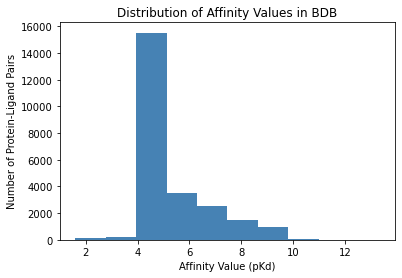
\includegraphics[width=0.5\linewidth]{chapters/datasetpreparation/figures/bdb.png} 
    \caption{Distribution of binding affinity values in BDB.}
    \label{fig:bdb}
\end{figure}

BDB dataset consists of 5 different setups for training and evaluating the model performance. To evaluate the performance of DeepDTA, we trained DeepDTA model with the knowledge derived from heterogeneous networks on five training setups of BDB dataset \cite{ozccelik2021chemboost}, and test the models in the corresponding test sets. 
\section{DrugBank}
DrugBank \cite{wishart2006drugbank, wishart2008drugbank, wishart2018drugbank} is an online database of information about drugs and drug targets. It contains information about drugs, such as chemical, pharmacological, and pharmaceutical data, and information about drug targets, such as sequence, structure, and pathways, as both bioinformatics and cheminformatics sources. Statistical information as of January 2021 is given in Table 
\ref{tab:drugbank_stats}. 14.350 drugs and 2.682.158 drug-drug interaction information from DrugBank were compiled as data within the scope of the project.

\begin{table}[]
\caption{DrugBank statistics (01.2021).}
\centering
\begin{tabular}{|l|l|}
\hline
\multicolumn{1}{|c|}{\textbf{Data}}  & \multicolumn{1}{c|}{\textbf{Number}} \\ \hline
Total Number of Small Molecule Drugs & 11.834                               \\ \hline
Total Number of Biotech Drugs        & 2.481                                \\ \hline
Total Number of Drugs                & 14.315                               \\ \hline
\end{tabular}
\label{tab:drugbank_stats}
\end{table}
\section{SIDER}

SIDER \cite{kuhn2010side, kuhn2016sider} is a database of drugs that have entered the market and their recorded adverse drug reactions extracted from public documents and prospectuses. Information such as side effect frequency, drug and side effect classification, and drug-target relationships are presented in a computer readable format. SIDER uses the Anatomical Therapeutic Chemical (ATC) Classification System, which is a drug classification system that classifies the active substances of drugs according to the organ or system they act on and their therapeutic, pharmacological and chemical properties. Side effects are coded by converting to MedDRA terminology. The current statistics of the data in the database are shown in Table \ref{tab:sider_stats}. From these data, 5,868 side effects and 139,756 drug-side effect relations were compiled within the scope of this thesis.

\begin{table}[]
\caption{SIDER Database statistics (10.2015).}
\centering
\begin{tabular}{|l|l|l|}
\hline
\textbf{Side Effects} & \textbf{Drugs} & \textbf{Drug-Side Effect Pairs} \\ \hline
5.868        & 1.430 & 139.756 \\ \hline
\end{tabular}
\label{tab:sider_stats}
\end{table}
\section{Comparative Toxicogenomics Database}
The Comparative Toxicogenomics Database \cite{davis2021comparative}, CTD, is a database that provides information on manually curated chemical–gene/protein interactions, chemical–disease and gene–disease relationships. CTD has several categories of data. These are chemicals, diseases, chemical-disease relationships, and gene-disease relationships. Statistical data as of February 2021 are given in Table \ref{tab:ctd_stats}. From these data, a total of 2.958.797 chemical-disease relationship and 28.253.189 gene-disease relationship data were compiled within the scope of the project.

\begin{table}[]
\caption{CTD statistics (02.2021).}
\centering
\begin{tabular}{|l|l|}
\hline
\multicolumn{1}{|c|}{\textbf{Data}} & \multicolumn{1}{c|}{\textbf{Number}} \\ \hline
Chemicals                  & 16.572                      \\ \hline
Diseases                   & 7.246                       \\ \hline
Chemical-Disease Relation  & 2.958.797                   \\ \hline
Gene-Disease Relation      & 28.253.189                  \\ \hline
\end{tabular}
\label{tab:ctd_stats}
\end{table}
\section{PubChem}
PubChem is an open chemistry database that contains small molecules, nucleotides, carbohydrates, lipids, peptides, and chemically-modified macromolecules, as well as information on chemical structures, identifiers, chemical and physical properties, biological activities, patents, health, safety, and toxicity data about them. Current statistics in the database are given in Table \ref{tab:pubchem_stats}.

\begin{table}[]
\caption{PubChem statistics (02.2021)}
\centering
\begin{tabular}{|l|l|}
\hline
\multicolumn{1}{|c|}{\textbf{Data}} & \multicolumn{1}{c|}{\textbf{Number}} \\ \hline
Compounds                           & 109.487.163                          \\ \hline
Substances                          & 270.034.522                          \\ \hline
Proteins                            & 96.280                               \\ \hline
Genes                               & 89.655                               \\ \hline
\end{tabular}
\label{tab:pubchem_stats}
\end{table}

 

\section{Universal Protein Resource}
The Universal Protein Source (UniProt) \cite{uniprot2021uniprot}, is an important resource for accessible protein information including protein sequence and functional information. As of June 2021, the total number of entries is 565.254  according to current statistics. 

\section{STRING}
Search Tool for the Retrieval of Interacting Genes/Proteins, STRING \cite{szklarczyk2021string}, is a biological database of known and predicted protein-protein interactions. The interactions include direct (physical) and indirect (functional) associations; they stem from computational prediction, from knowledge transfer between organisms, and from interactions aggregated from other (primary) databases.

The STRING database compiles information from several sources such as computational prediction methods, public text collections, laboratory experiments, and other databases. According to the statistics provided as of August 2021, the STRING database contains 67.592.464 proteins and 296.567.750 interactions at highest security (score $>=$ 0.900),  834.790.438 interactions with high security or better (score $>=$ 0.700), medium security or better 3.112.520.562 interactions (score $>=$ 0.400), and a total of 20,052,394,041 interactions.
\section{ChEMBL}
ChEMBL \cite{davies2015chembl, gaulton2017chembl} is a manually curated chemical database of molecules with drug-like properties and biological activity which is maintained by the European Molecular Biology Laboratory (EMBL). The ChEMBL database contains bioactivity data of pharmaceutical active ingredients which are reported with Ki, Kd, IC50 and EC50 values. ChEMBL examines how small molecules interact with target proteins, and how these compounds affect cells and whole organisms. Moreover, ChEMBL includes information about the 2D structure, calculated molecular properties, and the ADMET properties, which are assessment of in vivo absorption, distribution, metabolism, excretion and toxicity of small molecules. According to the statistics as of May, 2020, there are 1.941.412 chemicals in the ChEMBL database.
\section{Data Assembling}

Our idea was to represent chemicals and proteins better. Therefore, we compiled chemical and proteins related data from several online databases. And the challenging task was to assemble these compiled large data. For that purpose we analyze the available information in above mentioned databases and and map related information using common data. 

\subsection{Chemical Related Information}
DrugBank, PubChem, and ChEMBL databases are the main resources of chemicals and we mainly focus on them. As an initial step we compile 14.350 drugs from DrugBank and retrieve their DrugBank IDs and InChi (International Chemical Identifier) Keys. Using InChI keys, we map the data in DrugBank to PubChem and ChEMBL databases and able to get the information about 10.935 distinct drugs. With 10.935 drugs, we extract 2.196.820 drug-drug relation information from DrugBank database. Using the PubChem CID (Compound ID number) information available at PubChem database, we map the PubChem to SIDER and CTD databases. From SIDER database, we extract 5452 distinct side effects and 115.871 drug-side effect association information for 1003 drugs. From CTD database, we extract 7086 distinct diseases and 995.654 drug-disease association information for 3387 drugs. Finally, using the InChI keys, we map DrugBank to ChEMBL and compile SMILES (Simplified molecular-input line-entry system) representations of 10.935 drugs. 

\subsection{Protein Related Information}
UniProt and STRING databases are main resources used in this thesis. We compile 505.250 proteins from the UniProt database and more specifically we compile 202.160 proteins belonging to the Homo sapiens, as well as their amino acid sequences. Using the UniProt ID from UniProt database, we map 18.876 proteins to STRING database, and extract 183.746 protein-protein interaction information. Finally, using the UniProt ID and Entrez Gene ID we map UniProt database to CTD and extract 32.495 protein-disease association information for 32.169 proteins and 126 distinct diseases.
%assembling a het database

\chapter{BIOMOLECULE REPRESENTATION LEARNING FROM HETEROGENEOUS NETWORKS}

\chapter{EMPOWERING HETEROGENEOUS DATA WITH BIOMOLECULAR LANGUAGE}
\chapter{CONCLUSION}
#\label{chapter:experiments-and-results}

%Always place some text after headings before putting a graphics into
%a section as seen in Figure \ref{fig:sample}. 
\begin{figure}[htbp]
\begin{center}
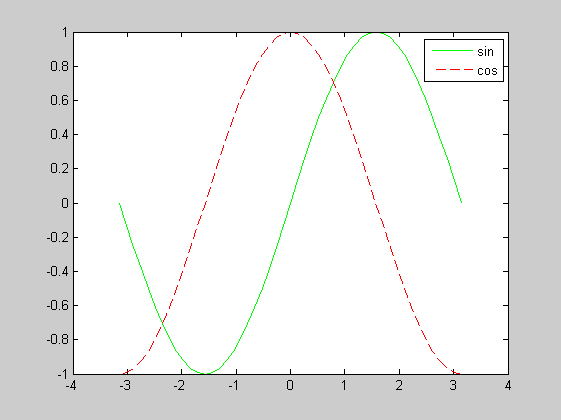
\includegraphics[width=0.5\columnwidth]{sample_figure.png}
\end{center}
\caption{Sin and
Cosine.}
\vskip\baselineskip % Leave a vertical skip below the figure
\label{fig:sample}
\end{figure}

Now, let us cite some studies: one source as \cite{doebelin},  two
sources as \cite{doebelin,exoplanetwebsite} or you may cite three or
more sources as 
\cite{doebelin,exoplanetwebsite,aran2007databaseofnon-manual}.\nocite{
liudissertation} \nocite{paper-IAT-2006-labels}
Observe that they are ordered in the references chapter in the same
order as
they are cited. Let us put a sample table as seen in Table
\ref{table:sample}. Please pay attention that the caption is followed
by a period.

\begin{table}[thbp]
\vskip\baselineskip 
\caption[Sample table]{Sample table.}
\begin{center}
\begin{tabular}{|c|c|c|}\hline
 & \textbf{Header 1}& \textbf{Header 2}\\\hline
\textbf{Row 1} & Bla bla bla& Bla bla bla \\\hline
\textbf{Row 2} & Bla bla bla  & Bla bla bla \\\hline
\end{tabular}
\label{table:sample}
\end{center}
\end{table}



Footnotes should be avoided as possible. If there is an absolute
necessity, footnotes should be used as this.\footnote{Example of a
footnote}

Item lists may be represented as follows:

\begin{itemize}
 \item This is an item. Do not use boldface for the items.
\begin{enumerate}
 \item This is a sub-item. Subsub-items are not allowed.
\end{enumerate}
\item Another item.
\end{itemize}
%  \item 
% \end{enumerate}
Item lists may also be represented as follows:
\begin{enumerate}
 \item This is another enumerated item.
\begin{itemize}
 \item This is another sub-item.
\end{itemize}

\end{enumerate}

\begin{thm}
The solutions of the equation $ax^2+bx+c=0$ with $a\neq 0$ are
$$
x=\frac{-b\pm \sqrt{b^2-4ac}}{2a}
$$
\end{thm}


\begin{proof}
We use the method of completing the square to rewrite $ax^2+bx+c$.
\begin{align*}
ax^2+bx+c&=a\left( x^2 + \frac{b}{a}x+\right)+c \\
  &=a\left( x^2 + \frac{b}{a}x+ \left(\frac{b}{2a}\right)^2
     -\left(\frac{b}{2a}\right)^2 +\right)+c \\
  &=a\left( x+\frac{b}{2a}\right)^2 - 
a\left(\frac{b}{2a}\right)^2+c\\
  &= a\left( x+\frac{b}{2a}\right)^2- \frac{b^2-4ac}{4a}.
\end{align*}
Therefore $ax^2+bx+c=0$ can be rewritten as 
$$
a\left( x+\frac{b}{2a}\right)^2- \frac{b^2-4ac}{4a}=0,
$$
which can in turn  be rearranged as
$$
\left( x+\frac{b}{2a}\right)^2= \frac{b^2-4ac}{4a^2}.
$$
Taking square roots gives
$$
x+\frac{b}{2a}= \frac{\pm \sqrt{b^2-4ac}}{2a}
$$
which implies
$$
x=\frac{-b\pm \sqrt{b^2-4ac}}{2a}
$$
as required.
\end{proof}
Finally, we will put a sample algorithm (PCA algorithm) using the
relevant package in a figure as shown in Figure \ref{alg:pca} and
sample equations.

\begin{figure}[htbp]
\label{alg:pca}
\begin{center}
\framebox[6.0in]{\begin{minipage}[t]{5.9in}
\begin{algorithmic}
\STATE
\STATE \textbf{Require}  $\mathbf{s_i},\ i=1,2,\dots,N$ are normalized
 
\STATE Compute the mean  $\mathbf{\bar{s}}$ using Eq. \ref{eq:mean};
\STATE Form the $N\times2L$ matrix $\mathbf{Q}$ as defined in Eq.
\ref{eq:q};
\IF{ $N < 2\times L$}
\STATE $\mathbf{Q} \Leftarrow \mathbf{Q}^T$ ;
\ENDIF
\STATE Compute the covariance matrix $\mathbf{C}_s$ using Eq.
\ref{eq:cov_matrix};\STATE Decompose $\mathbf{C}_s$
 to its eigenvectors   $\mathbf{e}_k$  and eigenvalues $\lambda_k$
satisfying Eq. \ref{eq:pca};
\IF{ $N < 2\times L$}
\FOR{$k=1$ to $K$}
\STATE $\mathbf{e}_k \Leftarrow \mathbf{Q}\mathbf{e}_k $ ;
\STATE $\mathbf{e}_k \Leftarrow \mathbf{e}_k/||\mathbf{e}_k|| $
(normalization);
\ENDFOR
\ENDIF
\STATE
\end{algorithmic}
\end{minipage}}
\end{center}
\caption[Principal Component Analysis Algorithm]{Principal Component
Analysis Algorithm.}
% \vskip
\end{figure}

\begin{align} 
\mathbf{\bar{s}} & =\frac{1}{N} \sum_{i=1}^N \mathbf{s}_i
\label{eq:mean}   
\\
\mathbf{Q} & =\left[ 
\begin{array}{cccc} 
 \mathbf{s}_1  - \mathbf{\bar{s}} & \mathbf{s}_2 - \mathbf{\bar{s}} &
\cdots & \mathbf{s}_N  - \mathbf{\bar{s}}
\end{array}
\right]_{2L\times N }
\label{eq:q}
\\ 
\mathbf{C}_s & =\frac{1}{N} \mathbf{Q}^T \mathbf{Q}
\label{eq:cov_matrix}
\end{align}

\begin{equation}
    \mathbf{C}_s \mathbf{e}_k = \lambda_k \mathbf{e}_k
    \label{eq:pca}
\end{equation}

\subsection{Example of First Subheadings}
Some text here
\subsubsection{Example of Second Subheadings}
Some text here too.
\chapter{CONCLUSION}
\label{chapter:conclusion}

The conclusions of the thesis should come
here.
% \nocite{NewEntry1,NewEntry2,NewEntry3,NewEntry4,NewEntry5,
% NewEntry6,
% NewEntry7,NewEntry8,NewEntry9,NewEntry10,NewEntry11,NewEntry12}

%\cite{*}
\bibliographystyle{styles/fbe_tez_v11}
\bibliography{references}

\appendix
\chapter{APPLICATION}
The appendices start here.

\end{document}